
\documentclass{report}

% PAGE DIMENSIONS
\usepackage{geometry}
\geometry{a4paper,margin=3.5cm}

% PACKAGES
\usepackage{graphicx} %support the \includegraphics command and options
\usepackage{fancyhdr} % Headers/footers (should be set AFTER setting up the page geometry and before hyperref)
\usepackage{color}
\usepackage{eso-pic} %background pictures
\usepackage[latin1]{inputenc}
\IfFileExists{inconsolata.sty}{% Use inconsolata as mono type if available
  \usepackage{inconsolata}%
}{}
\usepackage{csquotes}
\usepackage{booktabs} % for much better looking tables
\usepackage{tabularx}
\usepackage{array} % for better arrays (eg matrices) in maths
\usepackage{paralist} % very flexible & customisable lists (eg. enumerate/itemize, etc.)
\usepackage{verbatim} % adds environment for commenting out blocks of text & for better verbatim
\usepackage{alltt} %improved verbatim
\usepackage{titlesec} %to modify \chapter, \section, etc appearance
\usepackage{hyperref} %til links, email etc - giver ogs bookmarks i pdf filen
%\usepackage{dirtree} %directory trees
\usepackage{subfig} %make it possible to include more than one captioned figure/table in a single float
\usepackage{float} %float positioning etc
\usepackage{amsmath,amsfonts,amssymb,amsthm} %AMS' packages for symbols, theorems etc.
\usepackage{xfrac} %for slash fractions
%\usepackage{wrapfig}
\usepackage{multicol}
\usepackage{footnote}
\usepackage{perpage}
%\usepackage{ctable}
\usepackage[intoc]{nomencl} %for abbreviations list
\usepackage{listings} %for source code listings
\usepackage{marginnote} %Margin notes - use \marginnote{}
%\usepackage[textsize=footnotesize]{todonotes} %the ''disable'' option removes notes
\usepackage{url}
\usepackage{multirow}
\usepackage[normalem]{ulem} %underline, and variations thereof
%\usepackage[parfill]{parskip} %Activate to begin paragraphs with an empty line rather than an indent

% to justify typewriter monofont if used a lot in one place
\newcommand*\justify{%
  \fontdimen2\font=0.4em% interword space
  \fontdimen3\font=0.2em% interword stretch
  \fontdimen4\font=0.1em% interword shrink
  \fontdimen7\font=0.1em% extra space
  \hyphenchar\font=`\-% allowing hyphenation
}

% Define custom typewriter shorthands (uses \justify)
\newcommand{\custtt}[1]{\texttt{\justify{\small #1}}}
\newcommand{\smalltt}[1]{\texttt{{\small #1}}}

% Bibliography appearance
\usepackage[style=numeric,natbib=true,sortcites=true,block=space,backend=bibtex8]{biblatex}
\bibliography{content/bibliography}

% marginnote package options
\renewcommand*{\marginfont}{\color{red}\sffamily} %red, sans-serif
\reversemarginpar %margin notes on left side

% makes footnotes in tables possible (perpage package)
\MakePerPage{footnote}
\makesavenoteenv{tabular}

% listings package settings
\lstloadlanguages{Matlab,[ANSI]C}
\lstset{
  basicstyle=\ttfamily\small,
  %aboveskip=12pt,
  %belowskip=12pt,
  %frame=l,
  numbers=left,
  numberstyle=\ttfamily\tiny,
  numbersep=8pt,
  captionpos=b,
  tabsize=2,
  extendedchars=true,
  breaklines=true,
  showspaces=false,
  showtabs=false,
  keywordstyle=\color{blue},
  escapeinside={(*�}{�*)},
  %rangeprefix=,
  %rangesuffix=,
  includerangemarker=false,
  %stringstyle=\color{white}\ttfamily,
  %commentstyle=\color{white} %''cheat'' to hide comments
  xleftmargin=7pt,
  xrightmargin=7pt,
  %backgroundcolor=\color{lightgray},
  showstringspaces=false,
  morekeywords={step,impulse,pzmap,bode,freqz}
}
%\renewcommand*\lstlistingname{Code}

% hyperref package settings
\hypersetup{
  unicode=true,          % non-Latin characters in Acrobat�s bookmarks
  pdftoolbar=true,        % show Acrobat�s toolbar?
  pdfmenubar=true,        % show Acrobat�s menu?
  pdffitwindow=false,     % window fit to page when opened
  pdfstartview={FitH},    % fit page to the window Horizontal/Vertical
  pdftitle={TITLE},    % title
  pdfauthor={Alexander Adelholm Brandbyge, Frederik Hagelskj�r, Rudi Hansen, Leon Bonde Larsen, Kent Stark Olsen, Kim Lindberg Schwaner},% author
  pdfsubject={SUBJECT},   % subject of the document
  pdfkeywords={wordone} {wordtwo} {SDU}, % list of keywords
  pdfnewwindow=true,      % links in new window
  colorlinks=false,       % false: boxed links; true: colored links
  linkcolor=red,          % color of internal links
  citecolor=green,        % color of links to bibliography
  filecolor=magenta,      % color of file links
  urlcolor=cyan,           % color of external links
  plainpages=false
}

% Headers and footers
\pagestyle{fancy} % options: empty , plain , fancy
\setlength{\headheight}{15pt}
%\lhead{\nouppercase{\rightmark}}
\lhead{\nouppercase{\leftmark}}
\chead{}
%\rhead{}
\rhead{\nouppercase{\rightmark}}
\lfoot{}
\cfoot{}
\rfoot{\thepage}

\fancypagestyle{plain}{% Using the plain-style to be able number pages, but with an empty header! (using the report document class makes this nearly obsolete)
 \fancyhf{}
 \renewcommand{\headrulewidth}{0pt}
 \fancyfoot[RO]{\thepage}
}

% Widow/orphan penalties
\widowpenalty=300
\clubpenalty=300

%%% Contents appearance
\usepackage[]{tocbibind} % Put the bibliography in the ToC (Opts: nottoc,notlof,notlot)
\setcounter{tocdepth}{3} % set how many levels the table of contents displays. default=3
\usepackage[titles,subfigure]{tocloft} % Alter the style of the Table of Contents

% \includegraphics default folder
\graphicspath{{content/graphics/}}

% Number by section
%\numberwithin{equation}{section}
%\numberwithin{figure}{section}
%\numberwithin{table}{section}

% Paragraphs (handled by the parskip package currently?)
%\setlength{\parindent}{0pt}
%\setlength{\parskip}{2ex plus 0.5ex minus 0.2ex}

% Float positioning control
\setcounter{topnumber}{2}
\setcounter{bottomnumber}{2}
\setcounter{totalnumber}{3}
\renewcommand{\topfraction}{0.85}
\renewcommand{\bottomfraction}{0.85}
\renewcommand{\textfraction}{0.15}
\renewcommand{\floatpagefraction}{0.4}

% Header colour
\definecolor{FrontpageHeadingColor}{RGB}{5,5,60}%Heading colour definition

% Chapter name formatting
\titleformat
  {\chapter}%command
  [display]%shape
  {\normalfont\huge\bfseries}%format
  {\normalfont\Large\scshape\chaptertitlename\ \huge\thechapter}%label
  {10pt}%sep
  {\Huge}%before

% make nomenclature and change its heading/toc text (see nomencl package)
\makenomenclature
\renewcommand{\nomname}{Abbreviations}
%
%  * Pass this line to MakeIndex:
%    %bm.nlo -s nomencl.ist -o %bm.nls
%
%  * Use \nomenclature{abbr}{discriptive text} to add an entry to the
%    abbreviations list (best done where the abbreviation first occurs in the text)
%  * Example:
%    \nomenclature{ADHD}{Attention Deficit Hyperactivity Disorder}

\begin{document}
%
% Front page
\pagenumbering{alph} %frontpage numbered with a letter
\begin{titlepage}%
\currentpdfbookmark{Front page}{front_page}%hyperref pdf bookmark
\AddToShipoutPictureBG*{%background picture
 \put(0,0){
  \parbox[b][\paperheight][b]{\paperwidth}{%\parbox[position][height][inner-pos]{width}{text}
   \vfill
   %\begin{flushright}
   \includegraphics[width=0.43\paperwidth,trim=110 0 0 0]{content/00_frontmatter/sdu_seal.pdf}%trim=l b r t
   %\end{flushright}
   \vspace*{2.9cm}
  }
 }
}
\begin{flushright}
\includegraphics[scale=0.73]{content/00_frontmatter/sdu_logo.pdf}
\end{flushright}
\vspace*{2.7cm}
%
%\textsf{\Large{\textbf{Gruppe 1}}}
%
%\vspace*{0.3cm}
\setlength{\extrarowheight}{1.5pt}
\begin{tabular}{@{}l l}
	\textsf{\large{311289}} & \textsf{\large{Alexander Adelholm Brandbyge}}\\
	\textsf{\large{251289}} & \textsf{\large{Frederik Hagelskj�r}}\\
	\textsf{\large{260387}} & \textsf{\large{Rudi Hansen}}\\
	\textsf{\large{150179}} & \textsf{\large{Leon Bonde Larsen}}\\
	\textsf{\large{040282}} & \textsf{\large{Kent Stark Olsen}}\\
	\textsf{\large{160788}} & \textsf{\large{Kim Lindberg Schwaner}}
\end{tabular}
\setlength{\extrarowheight}{0pt}
\vspace*{1.5cm}
\\
\textsf{\Huge{\textbf{\textcolor{FrontpageHeadingColor}{Overskrift}}}}
\vspace*{0.5cm}
\\
\textsf{\Large{\textbf{\textcolor{FrontpageHeadingColor}{Underoverskrift}}}}
\vfill
\textsf{\\Faculty of Engineering\\
University of Southern Denmark\\
Niels Bohrs All� 1\\
5230 Odense M\\
Denmark}
\vspace*{10pt}
\\
\textsf{www.sdu.dk/tek\\
+45 6550 7303\\
tek@tek.sdu.dk}
\end{titlepage}%

%
% Abstract (un-numbered chapter)
\pagenumbering{roman} %until main content we use roman page numbering
\chapter*{Abstract}\addcontentsline{toc}{chapter}{Abstract}

The purpose of this project is to create a pan-tilt device, which position is to be regulated. A model of the pan-tilt system will be developed and a regulation system will be created for it. The device is moved by two dc motors, which are controlled by a FPGA, which also tracks speed and position. The FPGA is a Spartan3E, on a Xilinx Nexys 2, which will be programmed in VHDL. The system is regulated by an ARM microprocessor and the ARM is also taking care of the user interface. The ARM is a Stellaris LM3S6965 on an Evaluation Board programmed in C and a FreeRTOS OS is running on the system. The two units are communicating by a SPI connection. The team decided to divide the project into small independent modules. This will result in a high cohesion which will make modifications much easier to implement and earlier developed modules can be reused in the development, debugging and testing of other modules.
%
% Preface (un-numbered chapter)
\chapter*{Preface}\addcontentsline{toc}{chapter}{Preface}
This report was made during our fourth semester on the way to becoming engineers. The group has worked 
together to fine results on third semester, and thus agreed on some things we wanted to change compared 
to that. 

The first change was, that instead of going for the ``overkill'', we wanted to focus on finishing the 
project. We all have access to lots of practical work in our spare time projects, so in this project we 
wanted to go into the engineering skills in depth.
Individually we wanted to explore working in new areas and to dig deep and specialize. Therefore we 
wanted to split the project into smaller, more manageable parts and the participants in the group then 
picked their task of interest.

We agreed, that the system should be thoroughly tested, keeping in mind the difference between testing 
and debugging. Since a system can only be tested once it performs, our priority was to achieve a fully 
working and well documented system.

On the former semesters, different models for group corporation has been tried out and though 
interesting, the group felt a need to abandon the fine models and instead go for mutual reliance and 
trusting, that we are all working for a joint purpose. This meant that the advanced management tools and 
role based models were replaced by a simple log, and a will to finish the project.

All this together formed a decision about keeping the project simple and not decide on the application of 
the system, but simply build a robust and well performing system ready for others to facilitate.
We believe to have succeeded in these objectives.

\vspace*{0.5cm}
\begin{flushright}
Kent, Rudi, Kim, Alexander, Frederik and Leon
\end{flushright}
%
% Table of contents, figures, tables, listings and abbreviations
\tableofcontents
\listoffigures
\listoftables
\lstlistoflistings\addcontentsline{toc}{chapter}{Listings}
\printnomenclature[1.5cm]
%
% MAIN CONTENT
\clearpage
\pagenumbering{arabic} %''normal'' arabic numbering from here on out
%
\chapter*{Temp: Writing conventions}\addcontentsline{toc}{chapter}{Writing conventions}
For your eyes only
\section*{Naming conventions}
This is a list of how to write names of things

\begin{description}
  \item[PortAudio] is how they spell it at \url{http://www.portaudio.com/} \begin{quote}''PortAudio is a free, cross-platform, open-source, audio I/O library.''\end{quote}
  \item[Boost] is spelled Boost: \begin{quote}''Boost provides free peer-reviewed portable C++ source libraries''\end{quote}
\end{description}

\section*{\LaTeX\ references}
If one writes a reference to a \emph{specific} Figure, Table, Chapter or similar, they are written with a capital letter. For example:
\begin{verbatim}
To see how a figure looks, see Figure \ref{fig:label}
\end{verbatim}
eller
\begin{verbatim}
To read the first chapter, go to Chapter \ref{cha:chapter_one}
\end{verbatim} %THIS IS A TEMPORARY HELP TO WRITING (naming conventions and possibly other stuff)
%
\chapter{Introduction}\label{chap:intro}

This project is devised as a part of the B.Sc. Robot Systems Engineering, 4th term course at the Faculty of Engineering, University of Southern Denmark, Odense spring 2012. The implicit goal is to obtain basic knowledge of embedded systems. This is because embedded systems figure as a significant part of robots as these systems often controls actuators and process sensor inputs for controlling the robot. Therefore it is also demanded for students participating in this course to grasp the basic concepts of classic and modern control theory. Coupling control theory and embedded systems demand understanding of the basics of real time systems, digital systems, embedded systems and control systems. Applying this knowledge in the real world will be as significant as grasping the concepts.

Because the DSMI\footnote{The Engineering Education Model of the University of Southern Denmark} model is used as a framework for this particular education, it is required for the students participating in this course to formulate a strategy for solving an assignment in teams.

\section{Project description}
The purpose of the project work is to construct a control system for the pan/tilt frame shown in figure \ref{fig:pantiltsystem}, so that it is possible to control it with one or more user inputs. For example a joystick, a keyboard, buttons or via commands from a computer. In addition the system should also provide the user with options for feedback of significant system parameters. This is to be prioritized in the project:
\begin{itemize}
  \item A system analysis and modelling of the individual elements of the system.
  \item Analysis and design of the regulation loops in Matlab and Simulink.
  \item Documentation of FPGA design and implementation.
  \item Documentation of the design and implementation of microprocessor program, including choice of operating system.
  \item Test and verification of the system.
\end{itemize}



It is up to the project group to choose the characteristics of the regulator system and the regulator loops.

\begin{figure}[htb]
	\centering
	\includegraphics[width=\textwidth]{graphics/pantiltsystem.png} %trim=l b r t
	\caption{The pan/tilt system.}
	\label{fig:pantiltsystem}
\end{figure}

\pagebreak
\section{Requirements}
The following conditions are set for the system:
\begin{itemize}
\item The controller must be implemented on a microprocessor.
\item SPI must be used as the method of communication between the microprocessor and the FPGA.
\item The FPGA must control the PWM signals to the motors.
\item The FPGA must be used to determine the motors positions through use of  their built-in encoders.
\end{itemize}
\section{Project description}
The purpose with the project work is to construct a Pan and Tilt system so that it is possible to control the system from one or more user inputs eg a joystick, a keyboard, buttons or via commands from a computer. In addition shall the system also give the user options for feedback of significant system parameters.

\begin{itemize}
\item A system analysis and modulation of the systems individual elements
\item Analysis and design of the regulation loops in Matlab and Simulink
\item Documentation of FPGA design and implementation
\item Documentation of the microprocessor programs design and implementation, including division into tasks and selection of scheduling
\item Test and verification of the system
\end{itemize}

It is up to the project group to chose the regulator system og the regulator loops' characteristics.

\section{Requirements}

The following conditions are set for the system:
\begin{itemize}
\item The regulators' must be implemented on a microprocessor
\item SPI must be used in communication between the microprocessor and the FPGA
\item The FPGA shall control the PWM signals to the motors
\item The FPGA shall be used to determine the motors position via the encoders.
\end{itemize}

\section{The physical system}

The following is provided for the project:

\begin{itemize}
\item 2 pc. Pan and Tilt setup, that is to be shared between the project groups.
\item Motor with built in encoder to every project group
\item Print with double H-bridge to every project group
\end{itemize}

For the rest of the system the following devices are used:

\begin{itemize}
\item The microprocessor is a Stellaris LM3S6965 on an Evaluation Board, which is mounted on a
\item All hardware for user interface is from the given ARM test board.
\item The FPGA is a Xilinx Nexys 2 board with a Spartan-3E chip on board.
\item The SPI connection is made by connecting wires between ports on the to boards.
\end{itemize}

The pysical system was set up as following:


\chapter{Dynamics}\label{chap:dynamics}
This chapter will contain an analysis of the dynamics of the pan/tilt system which will result in a mathematical model. Calculations made throughout this chapter will reside in appendix \ref{app:dynamics_calc}. Identifying and understanding the relevant dynamics of a system is important as this will lead to an as accurate theoretical model as needed for the application. Ideally a perfect model would somewhat be preferred, but it would be a very difficult and tedious task to derive a perfect model and completely unnecessary to achieve. The reason for that is some of the dynamics are completely insignificant to the behaviour of the system, some other might have a little impact on the behaviour but can be omitted due to more dominating dynamic. The response of electrical circuits are often much quicker than the response of a mechanical system. This response delay is encoded into the poles of a system, which makes the poles of the system very interesting to analyse. The poles of the system tell if it is stable, and if any dynamic in the system possibly can be omitted due to its relatively fast response compared to the rest of the system which acts slower.

\section{Overview of pan/tilt}
The following will give an overview of the physical aspects of the pan/tilt system and also define the mathematics which is tied to the system. The pan/tilt is assembled from two motors, a set of gears connected to each motor. Each motor can rotate a mass individually by transferring torque from the motors, through the gears, to the masses which are connected to the gears. A model of the motors are needed, along with a model of the reflected inertia through the gears, and other dynamics might be relevant to, but are discussed later in this section.

\subsection{Motor}
The motor converts electrical energy to mechanical energy as a voltage is supplied to the motor. This voltage make the motor turn and this turning motion deliver torque though some gears to a mass which then spins up to some maximum speed. A simplification of a DC motors circuit can be seen in figure \ref{fig:motor_circuit}, from this a mathematical model of the motor can be derived.
\begin{figure}[htb]
	\begin{center}
	\includegraphics[scale=1,trim=0 0 0 0]{graphics/motor_circuit.pdf} %trim=l b r t (can cut off from every side)
	\caption{Simplification of circuit for a DC motor. Voltage supplied is denoted by $u$, $i$ is the current through the motor, $L$ is inductance, $R$ is resistance and $V_B$ is the the voltage generated from the coil rotating in a magnetic field.}
	\label{fig:motor_circuit}			% figure labels are of the form \label{fig:*}
	\end{center}
\end{figure}
Following can be derived from the circuit seen in figure \ref{fig:motor_circuit}.
\begin{align}
	u &= L\frac{di}{dt} +  Ri + V_B \Longleftrightarrow\\
	u &= L\frac{di}{dt} +  Ri + K_B\omega\label{eq:motor_model}
\end{align}
where $u$ is the voltage input, $i$ is the current, $\frac{di}{dt}$ is the time derivative of the current, $L$ is the inductance, $R$ is the resistance and $V_B$ is the voltage generated in the in coil of the motor as it spins in a magnetic field. $V_B$ can be expressed by $K_B$ which is the \textit{back-emf}\footnote{EMF is an abbreviation for electromotive force, which is the voltage generated from a coil rotating in a magnetic field.}-constant, times $\omega$, which is the angular velocity of the motor. As the motors need to move a mass an expression for torque is more interesting compared to the expression derived in \ref{eq:motor_model}. The electrical torque can be expressed in the following way:
\begin{equation}
	\tau = K_Ti\label{eq:electrical_torque}
\end{equation}
where $K_T$ is the torque constant.	The mechanical torque can be expressed in the following way:
\begin{equation}
	\tau = J_L\frac{d\omega}{dt}\label{eq:mechanical_torque}
\end{equation}
where $J_L$ is the inertial load on the motor, $\frac{d\omega}{dt}$ is the time derivative of the angular velocity of the motor. Equation \ref{eq:electrical_torque} and \ref{eq:mechanical_torque} equals each other if it is assumed that the energy is conserved in the transfer from electrical to mechanical torque, the following expression is obtained then obtained from equation \ref{eq:electrical_torque} and \ref{eq:mechanical_torque}:
\begin{align}
	K_Ti &= J_L\frac{d\omega}{dt} \Leftrightarrow\\
	i &= \frac{J_L}{K_T} \frac{d\omega}{dt}\label{eq:electrical_mechanical_torque}
\end{align}
To derive $\frac{di}{dt}$ the time derivative is taken of \ref{eq:electrical_mechanical_torque} which leads to:
\begin{equation}
	\frac{di}{dt} = \frac{J_L}{K_T} \frac{d^{2}\omega}{dt^{2}}\label{eq:electrical_mechanical_torque_derivative}
\end{equation}
Now \ref{eq:electrical_mechanical_torque} and \ref{eq:electrical_mechanical_torque_derivative} can be substituted into \ref{eq:motor_model} in which the following is obtained:
\begin{equation}
	u = \frac{L J_L}{K_T} \frac{d^{2}\omega}{dt^{2}} + \frac{R J_L}{K_T} \frac{d\omega}{dt} + K_B \omega
\end{equation}
%An expression for torque is needed, so the above equation is rewritten with respect to \ref{eq:mechanical_torque} which subsequently leads to:
%\begin{equation}
%	J_L \frac{d\omega}{dt} = \frac{K_T}{R} u - \frac{L J_L}{R} \frac{d^{2}\omega}{dt^{2}} - \frac{K_B K_T}{R} \omega\label{eq:torque_motor_model}
%\end{equation}

Stiction, coulomb and viscous friction are omitted as it is assumed that the inertia from the internal friction of the motor is a lot less than the inertia from the mass, so this concludes the model of the motor.

\subsection{Gears}
The gears does not add to the dynamics of the system but changes the existing poles of the existing system. Calculations for reflected inertia is kept in \ref{app:dynamics_calc}. 
  
\subsection{Precession}

\subsection{Omitted dynamic}

\section{State space}
\chapter{Low level control}\label{chap:llc}
Before the ARM core can control the physical system, an interpreting layer needs to be added, that can receive torque commands and control the physical system based on them, and report position and velocity of the physical system back as useful values.
This part of the system is situated on the FPGA, and architecturally, it is split in two nearly independent systems, one being the SPI driver and the other being the motor control.
The SPI driver acts as the link between the ARM processor and the FPGA and is described in chapter \ref{chap:comm}, the motor control section is described in this chapter.
The two subsystems communicate through a shared RAM block using the method described in chapter \ref{chap:comm}, but functions otherwise completely independent of each other.
No attempts to lock the RAM is made, even though race conditions can occur between the two sub blocks, they will exist for a very short time, as the SPI block transmits with one mHz and the RAM updates in 6 clock cycles, which is several magnitudes faster than the regulator task using these values.


\section{Motor interface}
The motor interface is responsible for presenting an easy to use interface to the arm processor, making it possible to control the motor torque and receive feedback in the form of pan and tilt position and velocity.
Also, an auxillary register is implemented, enabling the two parties to set and read flags between them, for instance the ARM can set the freerun bits, which disable the H-bridge entirely or command a reset of the position counters, the FPGA can report whether the index Hall sensors are active (meaning that the physical system approximately is in a neutral position).
All communication is done through the RAM block as seen on figure \ref{fig:FPGAMotorArchitecture}, thus the interface functions independently of the SPI implementation.

\subsection{Overall architecture}
The motor interface is split into two distinct parts. The PWM controller, which generates a PWM signal from a given input and a decoder controller, which reads the decoder pins, and tracks position and velocity.

A top level module is introduced to handle all memory interfacing. It houses all the individual component instances, and binds them together.

The output pins of the PWM controller A and B, is connected to the three pins of each H-bridge.
The input pins of the decoder system comes from the index pins of the hall sensors mounted on the pan/tilt system and the decoder A and B signal from the two output pins on the motors.

\begin{figure}[htb]
\centering
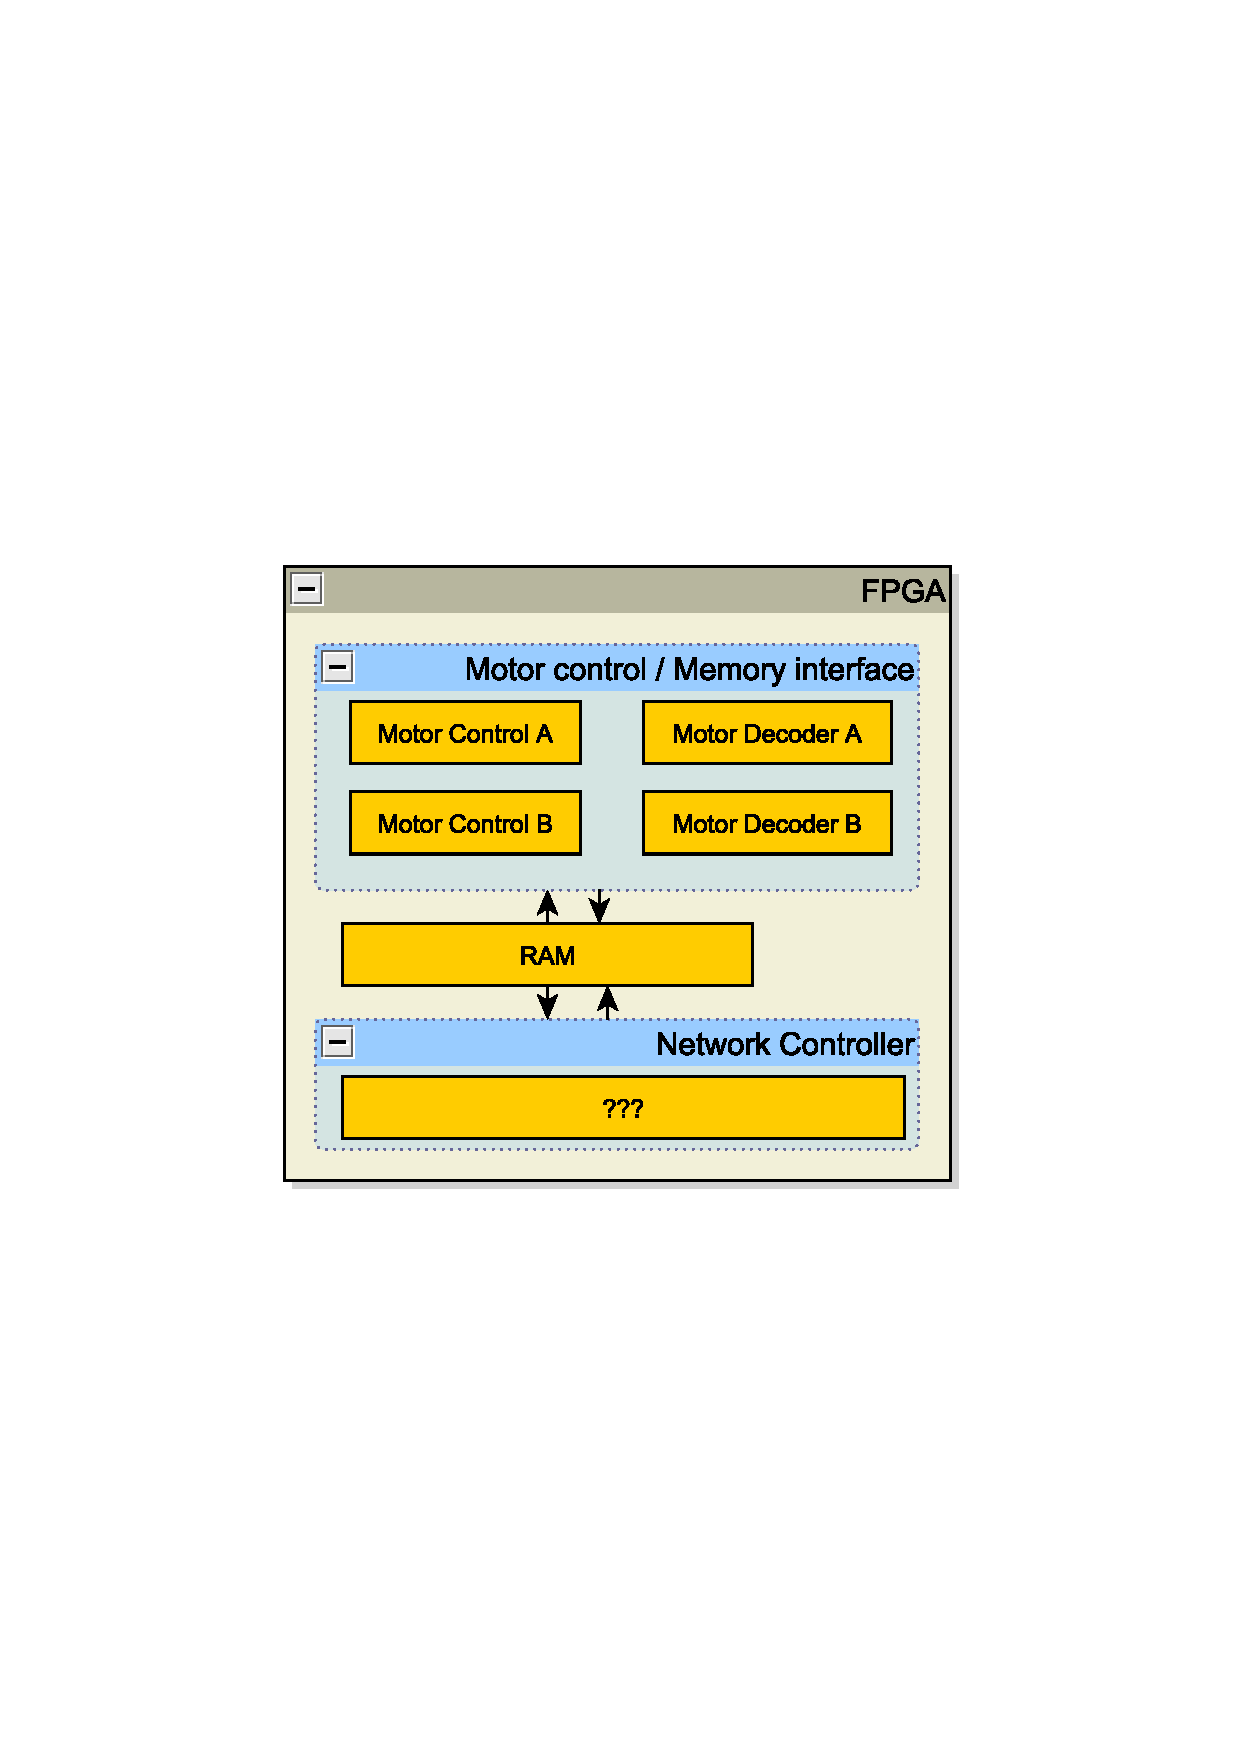
\includegraphics[scale=0.6,clip,trim=135 270 135 270]{FPGAmotorarchitecture.pdf}

\caption{FPGA architecture, from the motor interface perspective, it should function without concern for the SPI part of the system}
\label{fig:FPGAMotorArchitecture}
\end{figure}

\subsection{Memory layout}
The memory layout is as seen in table \ref{tab:Memorymapping}. The position is represented by an unsigned bit, centered at 0x8000, this is because it is easier to calculate the position without considering a sign, and it would make no difference for the control system on the arm whether the position is represented by signed or unsigned numbers.
Velocity output and duty cycle input is represented as a 16 bit signed twos-complement value.
This is because the sign bit makes it easy to read what the desired motor direction is.
The aux register reads position reset, and motor freerun command bits. It also sets two bits, representing whether the hall sensors indicate that the system is in zero position.



\begin{table}[htb]
\centering
\begin{tabular}{|l|r|}
\hline
Address & Value \\
\hline
0x02 & DUTY A MSB \\
0x03 & DUTY A LSB\\
0x04 & DUTY B MSB\\
0x05 & DUTY B LSB\\
0x06 & POS A MSB\\
0x07 & POS A LSB\\
0x08 & POS B MSB\\
0x09 & POS B LSB\\
0x0a & VEL A MSB\\
0x0b & VEL A LSB\\
0x0c & VEL A MSB\\
0x0d & VEL A LSB\\
0x0e & AUX FROM ARM\\
0x0f & AUX TO ARM\\
\hline 
\end{tabular}
\caption{Memory locations of control registers}
\label{tab:Memorymapping}
\end{table}


\section{Motor control block}


The motor control block is split into 3 seperate modules.
The PWM generator, the signed-to-magnitude splitter, and the Motor AUX control as seen on figure \ref{fig:PWMblock}.
It takes a 16 bit signed integer and a control bit as input, indicating whether the motor should be driven by a PWM signal, or if it should be set in free run mode. 
When the motor is not in free run, the enable pin on the H-bridge is high, and the PWM signal changes between the braking and running state. If the free run bit is set, the H-bridge is disabled and no PWM signal is generated.

\begin{figure}[htb]
\centering
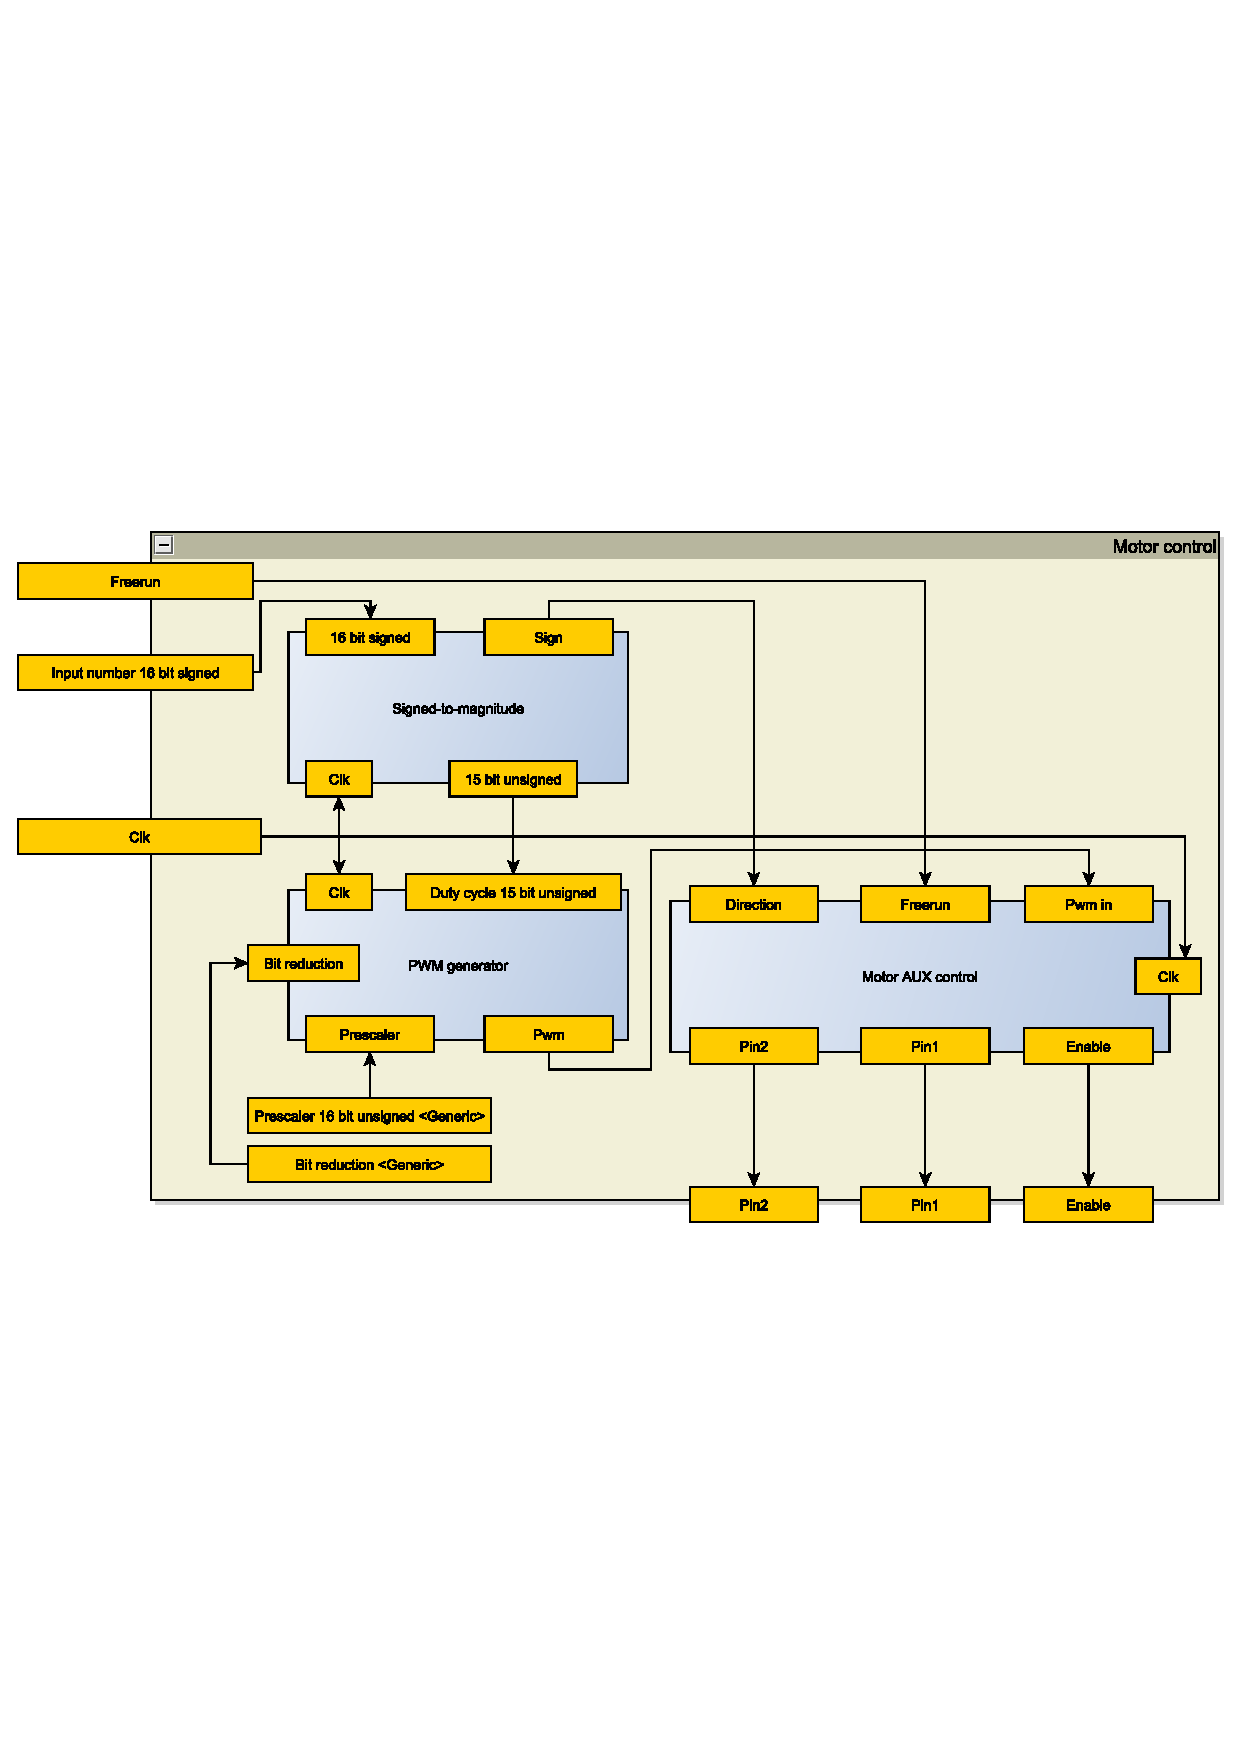
\includegraphics[scale=0.6,clip,trim=0 250 10 250]{PWMblock.pdf}
\caption{Block/signal layout of the Motor control block}
\label{fig:PWMblock}
\end{figure}

\subsection{PWM generator}
The PWM generator takes a clk signal and a duty cycle (15 bit unsigned value) as input. It also takes two generic parameters as input. A prescaler value to decrease the frequency, and a bit reduction parameter to increase it. These allows the PWM block to be configured for a desired frequency.

Internally the generator consists of a counter register that is decremented each tick as seen of figure \ref{fig:PWMchart}. If the counter is less than the input, the output is 1 otherwise it is zero.
If the counter value underflows, it is set to the second highest value it can represent. This ensure that the PWM block is able to output high and low value dc if needed, at the cost of lacking an extra bit of resolution.

The bit reduction parameter effectively reduces the amount of significant bits in the counter and value signals.
The prescaler is used to introduce a delay between each tick.

The frequency of the PWM needs to be at around 20khz or above. If it is lower than that it is in the audible range of frequencies which would be an annoyance. If the frequency is too high, to much energy is lost in the transistors, not to mention the fact that an h-bridge has a switching time, which would distort the actual duty cycle output.

For calculating the PWM frequency the following formula is used: 
\begin{equation}
F_{PWM} = \frac{F_{xtal}}{2^{number of bits}}
\end{equation}

Without using prescaler and bit reduction values, the PWM frequency is calculated with 16 bit resolution and a 50 mhz internal clock, which gives a resulting frequency:
\begin{equation}
\frac{50 mhz}{2^{15}} = 1525.88 hz
\end{equation}

This is way to low, and therefore the amount of used bits are reduced by four giving the frequency:
\begin{equation}
\frac{50 mhz}{2^{11}} = 24414.1 hz
\end{equation}
Which is just above the minimum frequency requirement.

\begin{figure}[htb]
\centering
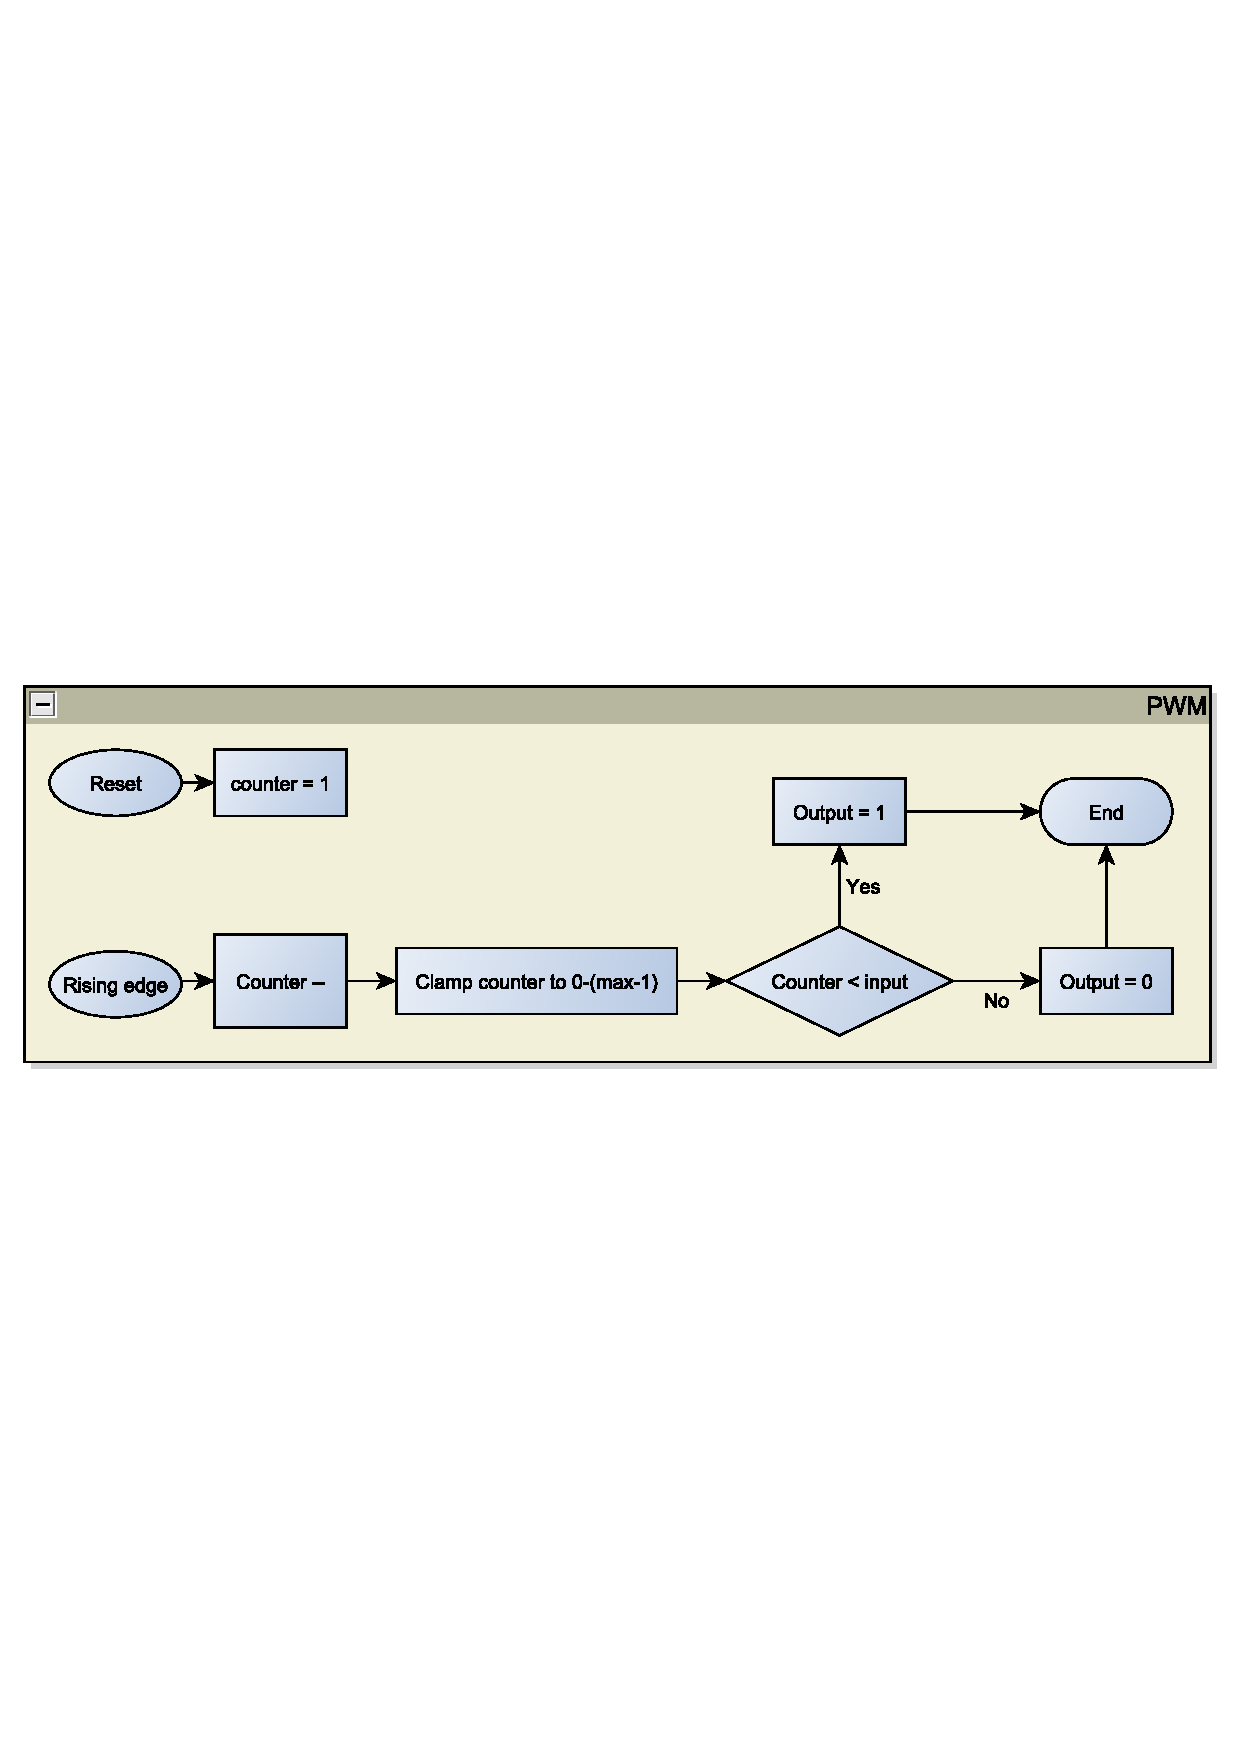
\includegraphics[scale=0.6,clip,trim=10 330 10 330]{PWMexecution.pdf}
\caption{Flowchart of the PWM generator}
\label{fig:PWMchart}
\end{figure}

\subsection{Signed-to-magnitude splitter}
The signed-to-magnitude splitter takes a signed 16 bit integer as input and outputs the sign and magnitude separately.
The magnitude is computed as follows:
If it positive, its just the 15 last bits, if it is negative the twos compliment value is the output.

\subsection{AUX control}
The aux control takes the direction, PWM and freerun signals as input, and output the PWM signal on either pin 1 or 2 of the h-bridge. If the freerun pin is not high, the enable pin is high, if the freerun pin is high, no PWM is output, and the enable pin is low.

\section{Decoder system}
The decoder system is responsible for reading the state of the pan/tilt system from the hall sensors mounted on the system, and the quadrature encoders on the motors. 
It outputs a relative position from the reset point and a velocity for each of the two axes, as precise as possible.

The decoder is split into 4 major components: The Input filtering, the quadrature decoder, position normalizer and velocity estimator components, as seen on figure \ref{fig:decoderblock}. 



\begin{figure}[htb]
\centering
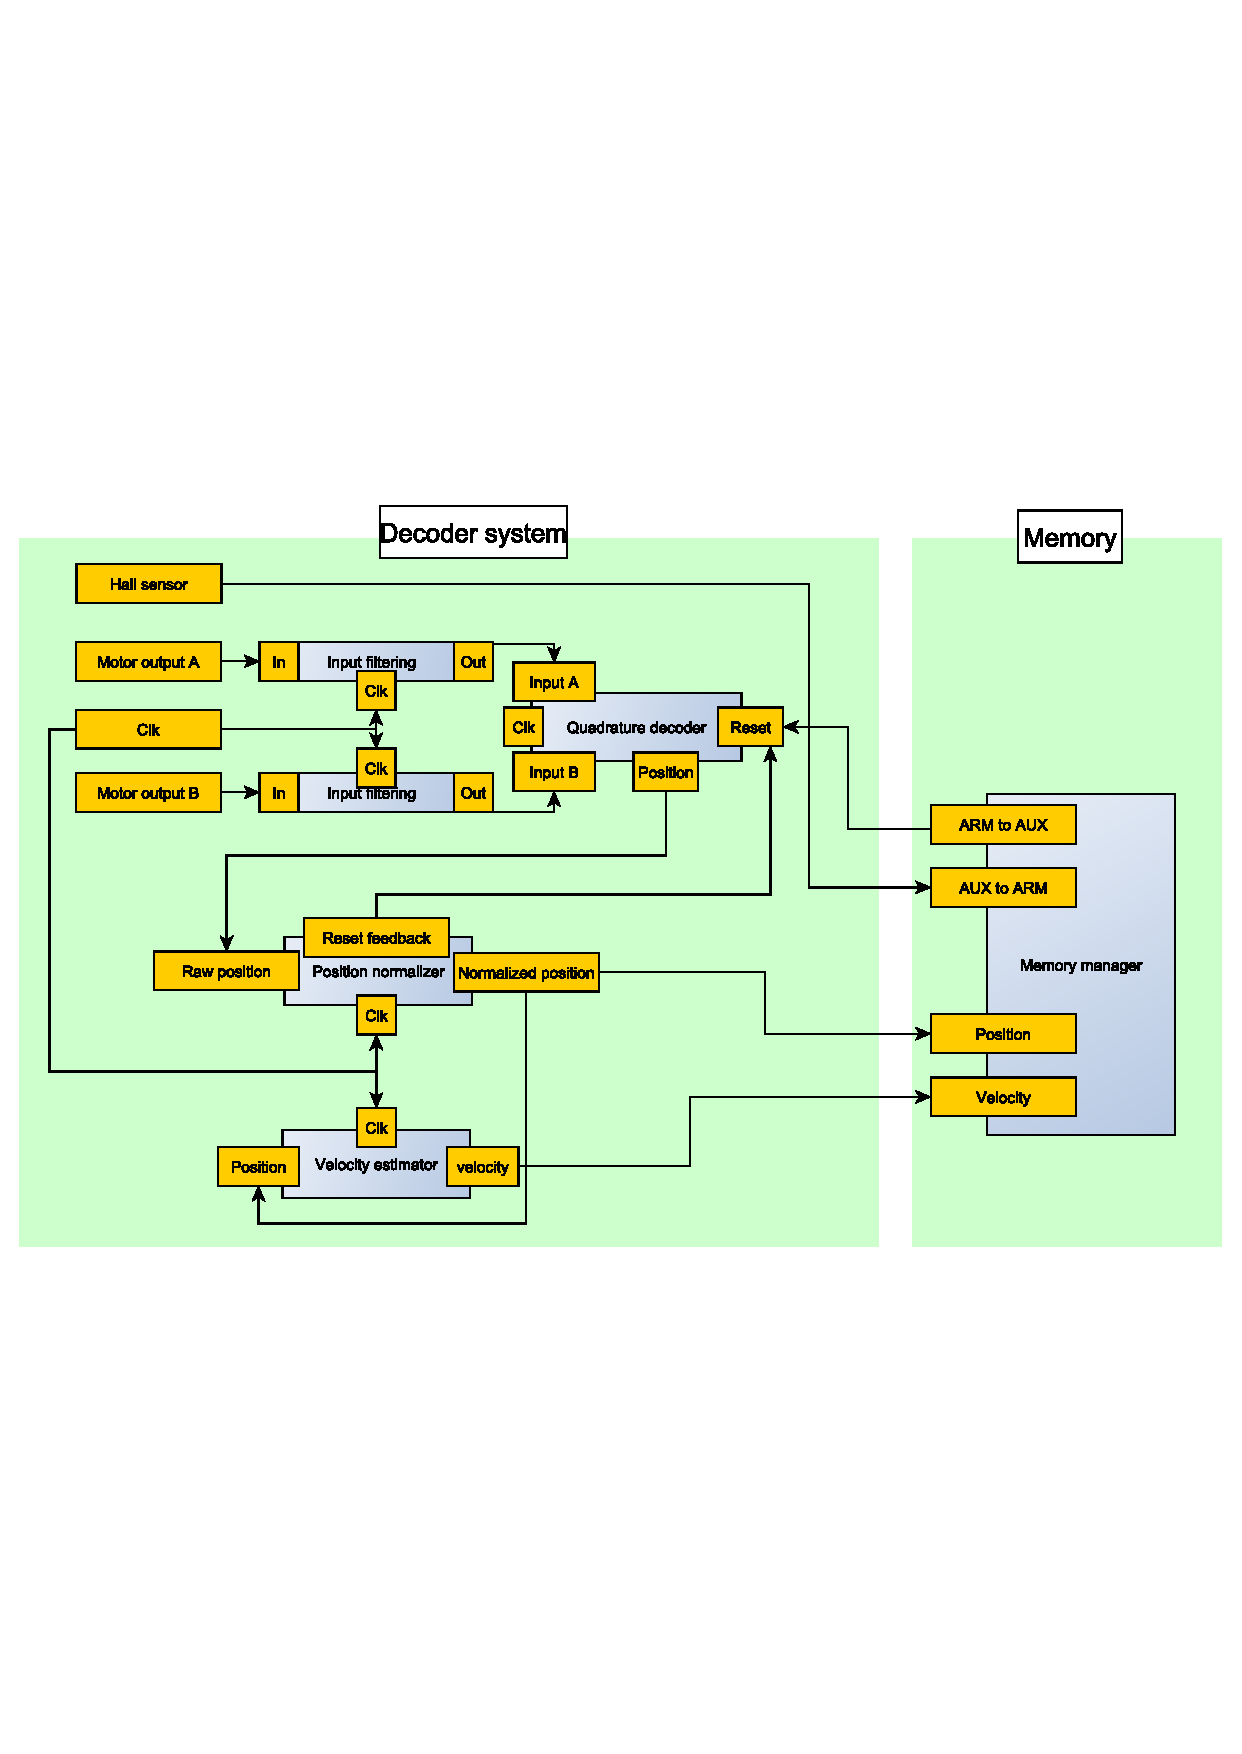
\includegraphics[scale=0.6,clip,trim=2 250 2 230]{decoderblock.pdf}
\caption{Block/signal layout of the decoder system}
\label{fig:decoderblock}
\end{figure}


\subsection{Input filtering}
Since the input signal comes from the world outside the FPGA, unwanted noise must be removed for it to be used. However, the regulator depends on this signal, so care must be taken not to introduce an unwanted large delay, as that would make the signal  useless.

To remove noise, a simple debounce, with hysteresis is applied, it features a counter that, for every clock pulse counts up if the input signal is high and down if it is low.
When ever the counter rises above a threshold, and the filter is outputting a low signal, it changes to high. The same opposite when counting down.
The counter part of the process introduces a delay in output changes, so that a lot of switching back and forth between high and low, will not affect the output. The hysteresis helps negate short burst errors in the input. 

The difference between the hysteresis counters lowest value and the rising edge value, or the highest value and the falling edge value, whichever is highest, determines the maximum frequency the input filter will let through, as well as the delay introduced in the position counter.

A set of values must be chosen that filters the signal adequately, without producing error signals. The tilt rotor has been observed to have approximately 1000 ticks pr. full revolution, and with full power to the motors, max one rotation pr. second.
This means that the input filter should be able to let a 1khz signal through at least. \\ 
Since external forces can temporarily push the system to higher frequencies, it is assumed that a max frequency of 1mHz should cover all but the most extreme cases.

This means that the maximum input delay can be 50 clock ticks.
In this assignment, a set of values was then chosen within the constraints: 
Lowest value: 0
Maximum value: 20
Low hysteresis: 4
High hysteresis: 16

These values give a maximum input delay of 16 clock ticks(320 ns) which is sufficient for this application.

\subsection{Quadrature encoder}
The quadrature encoders job is to convert the two decoded signals from the motor, to a relative position. The signal is generated from two hall sensors that are positioned 90 degrees apart. Giving 4 different output states, each state indicating what quadrant the motor is positioned in, an example of the signal can be seen in figure \ref{fig:decodersignal}.
\begin{figure}[htb]
\centering
\includegraphics[scale=0.6,clip,trim=0 0 0 0]{ddecodersignal.pdf}
\caption{Example decoder output from a motor with constant speed}
\label{fig:decodersignal}
\end{figure}
The decoding process can be thought of as a state machine (with the encoder output being the state variable), where a state transition corresponds to a movement step in one of two directions.
When the decoder is first powered, a default position value is kept, and then incremented or decremented according to the statetransition. The default value is set at 0x8000 unsigned integer, as this allows for the maximal displacement in either direction. 
Overflow is not handled in this module, as it is not its job to know anything about the configuration the motor is in, however an external reset pin is provided, which returns the counter to 0x8000. (This reset signal is incidentally powered by the position normalizer module).
The situation where the input pins both change in one clock cycle is not handled by the system.

\begin{figure}[htb]
\centering
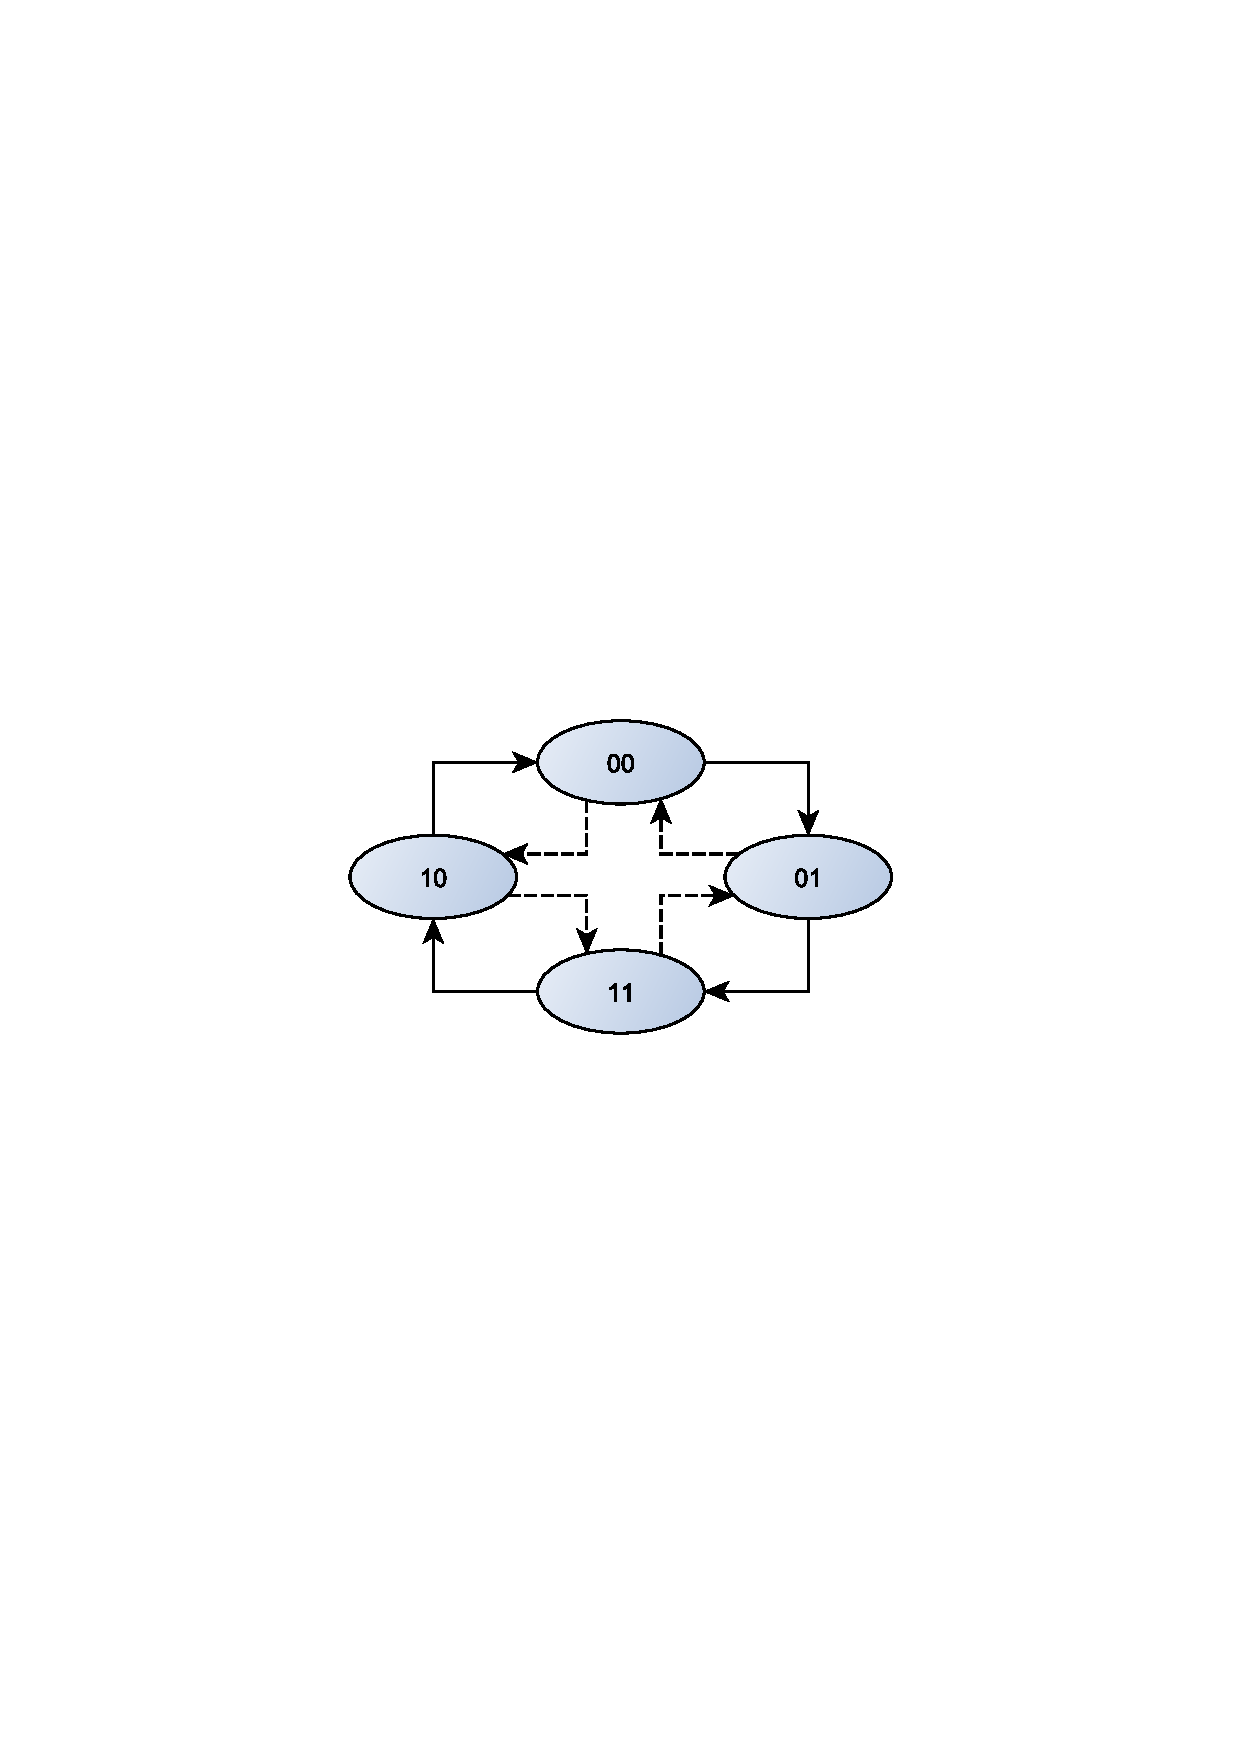
\includegraphics[scale=0.6,clip,trim=130 330 130 330]{decoderstates.pdf}
\caption{State diagram of the decoder module, the stipled arrows indicate a negative clockwise, the solid indicate a counter-clockwise or vice verca.}
\label{fig:decoderstate}
\end{figure}

\subsection{Position normalizer}
The position normalizer block is used for any conversions/adaptations of the raw position value necessary. For instance the position could be converted to radians or similar. It also features a feedback reset signal, if this should be necessary. 
In the final version of the application, this block does nothing other than let the input go directly to the output.
Should any automatic reset system be required, based on the position, this is the block to handle it.

\subsection{Velocity estimator}
The velocity estimator is responsible for measuring the velocity based on the counter input.
There are several methods available for measuring the velocity, each with its drawbacks and strengths.
A simple method is to compare the position with a fixed frequency, so that for instance each second, the velocity is the difference between the position before and after a second has passed. This has the advantage of being easy to implement and test, also everything is implemented with integers. The drawback is that this method can produce wildly varying velocity measurements, especially if the actual velocity produces a position change frequency just above or below the sampling frequency.
This drawback can be offset by \"tuning\" the sampling frequency until a desirable behavior has been reached.
Another method is the secant method, where the time between each change of the position is measured. The reciprocal of this is then the velocity. The advantage of this method is that it is, in theory, very precise. The drawback is that a floating/fixed point division is necessary, in order to obtain the correct result. Also should there be any imprecision in the motor decoding, it will be reflected strongly in the measured velocity. Furthermore, a time-out period must be included, for there is no edge to detect when the motors stop moving.

In both cases smoothing of the result can be needed. By using a running average filter, the velocity measurement can be smoothed over many samples, but a first order delay in the measurement is introduced.

In the final application, there is no velocity estimator, since it is not needed in the chosen regulation method, however the two mentioned measurement methods are included in the codebase for completeness sake.


\section{Watchdog}
Since all control commands are buffered in the RAM until updated to new values, the FPGA has no way of knowing if the commands are still valid commands or they are erroneous commands due to either the ARM processor crashing, or cable failure etc. This means that in case the case of failure, the FPGA it will continue outputting a PWM signal if any velocity command has been issued before the meaningful communication died. To correct this problem, a watchdog is implemented. It outputs an enable signal as long as there is a link between the FPGA and ARM, and the ARM routinely updates its assosiated register. 
To detect the link presence, two registers in the control register are constantly incremented, and the watchdog keeps a watch on them, should they fail to change within a set time, the watchdog will stop all motor activity and go to a velocity of zero.
The watchdog module is not included in the final application due to time constraints.

\section{Conclusion}
The individual blocks are tested and proven working, with the exception of the velocity estimators, in chapter \ref{chap:experiments} section \ref{sec:llctest}. This means that the FPGA motor control block meets all of the requirements, for it to be used in the control system. 

\chapter{Communication protocol}\label{chap:comm}
\chapter{Operating system}\label{chap:os}
\chapter{User interface}\label{chap:ui}
\chapter{Experiments}\label{chap:experiments}
\section{Performance testing}

\subsection{Precision of the system}\label{subsec:precisionofsystem}
This experiment will test the precision of the complete system with the
parameters found from simulating the system. The parameters can be found in
table \ref{tab:actual_gain_values}

\subsection*{Setup}

The test is performed by fastening a laser pointer on the pan/tilt system. A
board is placed next to the system and two positions where the pointer is on the
board are chosen as seen in figure \ref{fig:systemtestsetup}. The laser pointer is placed 180 cm
from the board. Thus each degree is at aproximately 3 centimetres wide.

\[ tan(1 \ deg) * 180 \ cm \approx 3,14 \ cm \]


\begin{figure}[htb] \centering \includegraphics[width=\textwidth,trim=0 0 0
0]{graphics/overallsystemtest.png} %trim=l b r t (can cut off from every side)
	\caption{Setup of the test. From left to right; the mounted laser, the system pointing at the board, laser dot and marks.}
	\label{fig:systemtestsetup}			% figure labels are of the form \label{fig:*}
\end{figure}

The system runs in automode and changes between two setpoints. The positions
are marked and the test ends after ten iterations. 

\subsection*{Results}

At both points the error was less than five centimetres and most of the time
less than two centimetres. This means that the system have an accuracy between 0.658 and
3.293 degrees. This precision is reached with overshoot.

\[ \frac{2,0 \ cm}{3,14\ cm/deg} = 0,64 \ deg \]

\[ \frac{10,0 \ cm}{3,14 \ cm/deg} = 3,19 \ deg \]

\subsection*{Conclusion}

The system itself, has a precision of af third degree.
\[ \frac{360}{160} = 1/3 \]

It is a high precision that have been observed, at times the uncertainty is as
small as the precision of the system. Though it does also show that a higher
precision can be obtained. Overshooting was though occurring in the control.
Additional tuning of the parameters might enhance the performance.

\subsection{Precision of new parameters}\label{sec:precisionofsystem2}

This experiment will test the PID values found in table \ref{tab:actual_gain_values}
under best performance.

Here the system will run in automode between two position but only one of the
positions are marked. This is repeated ten times.

\subsection*{Setup}

The setup is similar to the setup in section \ref{subsec:precisionofsystem}, see
Figure \ref{fig:systemtestsetup}, with the exception that only one point is measured and at
the distance 370 centimetres. Thus each degree is 6,46 centimetres wide.

\[ tan(1 \ deg) * 370 \ cm \approx 6,46 \ cm \]

\subsection*{Results}

In this test the precision of the pan and tilt were recorded to be quite
different. The vertical precision was 7,5 cm, but the horizontal precision was just 2,0 cm. Thus the pan/tilt system have
reached precision of respectively 0.31 degrees and 1.16 degrees.


\[ \frac{2,0}{6,46} = 0.31 \]

\[ \frac{7,5}{6,46} = 1.16 \]

\subsection*{Conclusion}
The pan has reached a constant precision on par with the system precision
of one third of a centimeter. The tilt part have also become more precise, but
it should be possible to make it even more precise. It could be that because the
tilt is affected by gravity it is harder to control than the pan.



\section{PID experiments}\label{sec:pid_experiments}


\section{SPI software}\label{sec:armspitest}

This experiment will test the precision of the complete system. 


\subsection{Test Setup}



\subsection{Result}


\subsection{Conclusion}


\chapter{Discussion}\label{chap:discussion}
The main approach in this project, has been to divide the assignment into specialized manageable tasks, with defined interfaces.  This has given each member of the group a chance to specialize in their given assignment area, without the need to worry about the larger picture of the project.

In this project, no practical application, fx a tracking system, was to be implemented using the system.
This made it the scope of this project to build an interface, to show the efficiency of the control system. Thus it was not possible to define all the systems requirements.

In contrast with previous projects, where the group have attempted to use responsibility based work models, specifically the Belbin model, this time an expertise focused model was used, where each individual group member primarily focused on their own practical field, and all other assignment were handled as they came naturally. 

Instead of having a lot of meetings, the group used a central log. This was an open Google document, where most of the  group communication took place. This freed up a lot of time, that would otherwise have been spent on meetings for the sake of coordination. And thus time could be, and was, used more constructively. The log could also guaranteed that each group member quickly could get a clear picture of the status of the project, and what small assignments were pending.

Even though the project resulted in a successful system, there have been several areas where improvements could be made. For instance the velocity estimators on the FPGA, together with the control model that used them.
Also some of the initial solutions proposed, turned out to be more than sufficient, but hard to implement, and therefore a simpler solution was implemented. The statespace model was proposed in the simulation chapter, but it ended up with a simple S-domain transfer function. These areas were all explored a bit, but was ultimately cut, due to the fact that it was prioritized to have a working system by the deadline, instead of a non working, but more advanced system.

Due to the architecture of the system having an extremely low coupling, additions and replacements could be easily made and interfaced, without requiring a complete redesign. The test of the CPU load also shows that a more complicated control algorithm could be implemented without requiring new hardware, or redesign of other modules.

test vs debug

arbejdsform
	forventninger: krav til 
	project forløb


pony

\chapter{Conclusion}\label{chap:conclusion}

%overall
A working system was created for the pan/tilt. 
%dynamics
A mathematical model was developed and analysed, it is concluded that using a state-space model for simulating the system is excessive, and a simple transfer function was used instead.
%control
A PID control model was made, that could accurately control the system.
%llc communication
A working motor interface was made for the FPGA and it was possible to control the system through an SPI link.

%ARM
%The control system was successfully implemented on the microprocessor together with the operating system handling all the different tasks. 

The operating system on the microprocessor could easily run the different tasks, including the control task, and still have more than half of its execution time available.


%FINAL SOLUTI--CONCLUSION!!!
Even though some parts were downgraded to meet the deadline, the system works and is very precise.
% 
% References
\clearpage
\nocite{*} % Includes all of the .bib content
\printbibliography\addcontentsline{toc}{chapter}{Bibliography}
%
% Appendix
\appendix %all sections below are numbered A, B, C,...
\chapter{Calculations for dynamics}\label{app:dynamics_calc}
This appendix will contain calculations for the chapter concerning dynamics of the system.

\section{Inertia of the pan/tilt}
A sketch of the pan/tilt system is shown in the figure below.
\begin{figure}[htb]
	\centering
	\includegraphics[width=\textwidth]{graphics/pan_tilt_sketch.pdf} %trim=l b r t (can cut off from every side)
	\caption{Simple sketch of the pan/tilt system with measurements. The dimension of the profile is 40 x 40 mm. The profile that is used weigh $1.565\sfrac{kg}{m}$.}
	\label{fig:pan_tilt_sketch}			% figure labels are of the form \label{fig:*}
\end{figure}

\subsection{Pan inertia}
To calculate the inertia of the pan mechanism some considerations have to be made about how to model it. Figure \ref{fig:pan_tilt_sketch}(a) will be modelled in a way so the bar connected to the turning shaft will be considered as a rod with two point masses connected to each end of the bar, the total inertia of the pan mechanism will be calculated from the parallel axis theorem. The parallel axis theorem says:
\begin{equation}
	J = J_{COM} + M d^{2} \label{eq:parallel_axis_theorem}
\end{equation}
where $J$ is the total inertia, $J_{COM}$ is the inertia of the base bar, $M$ is the mass that is displaced and $d$ is the displacement. $J_{COM}$ is calculated as follows:
\begin{equation}
	J_{COM} = \dfrac{M L^{2}}{12} \Longrightarrow J_{COM} = \dfrac{(1.565\sfrac{kg}{m} \cdot 0.42m) \cdot (0.42m)^{2}}{12} = 0.058 kg \cdot m^{2}
\end{equation}
Calculation of the total inertia is calculated as follows:
\begin{align}
J_{Pan} &= J_{COM} + 2 \cdot M d^{2} \Longrightarrow \\
J_{Pan} &= 0.058 kg \cdot m^{2} + 2 \cdot (1.565\sfrac{kg}{m} \cdot 0.246m) \cdot (0.21m)^{2} \Longrightarrow \label{eq:pan_inertia_temp} \\ 
J_{Pan} &= 0.092 kg \cdot m^{2}\label{eq:pan_inertia}
\end{align}
\ref{eq:pan_inertia_temp} has its second term multiplied with two, this is done as the pan mechanism has two masses that is displaced equally from the axis of rotation.

\subsection{Tilt inertia}
The inertia of the tilt part of the system is considered as a rod with two point masses displaced equally from the axis of rotation. The inertia is calculated the following way:
\begin{equation}
	J_{COM} = \dfrac{ML^{2}}{12} = \dfrac{2 \cdot 1.565 \sfrac{kg}{m} \cdot 0.293 m \ (0.293m)^{2}}{12} = 0.079 kg \cdot m^{2}
\end{equation}
Adding the displaced masses to the inertia is done with the parallel axis theorem as follows:
\begin{align}
J_{Tilt} &= J_{COM} + 2 \cdot M d^{2} \Longrightarrow \\
J_{Tilt} &= 0.079 kg \cdot m^{2} + 2 \cdot (1.565\sfrac{kg}{m} \cdot 0.280m) \cdot (0.145m)^{2} \Longrightarrow \label{eq:tilt_inertia_temp} \\ 
J_{Tilt} &= 0.097 kg \cdot m^{2}\label{eq:tilt_inertia}
\end{align}

\section{Gears}
The load at the motors are the reflected inertia through the gears plus the inertia of the rotor in the motor, the rotors inertia is omitted. The two gears are connected together and then connected between the motor and the inertia. The gearing system is equal on the pan and the tilt. Figure \ref{fig:app_gears} show a simplification of the gearing.
\begin{figure}[htb]
	\centering
	\includegraphics[scale=1,trim=0 0 0 0]{graphics/gears.pdf} %trim=l b r t (can cut off from every side)
	\caption{Simplification of the gears in the pan/tilt system. (a) Show a simplification of a planetary gear which has, according to the datasheet of the motor which is included on the CD, a gearing of $N = 30:1$. (b) The gearing of the belt driven gear is experimental measured and calculated to be $N = 1:3$.}
	\label{fig:app_gears}			% figure labels are of the form \label{fig:*}
\end{figure}
The load reflected through a gear is given by\footnote{REF NEEDED!!!   (http://www.techno-isel.com/tic/h834/PDF/H834P009.pdf)}:
\begin{equation}
	J_R = \frac{J_L}{N^{2}}
\end{equation}
where $J_R$ is the reflected load behind the gear, $J_L$ is the load in front of the gear, N is the gear ratio. As the pan and tilt gearing is equal the following expression is derived the total gearing between the motor and the mass:
\begin{equation}
	J_R = \frac{\frac{J_L}{(\sfrac{1}{3})^{2}}}{30^{2}} = \frac{J_L}{(\sfrac{1}{3})^{2} \cdot 30^{2}}\label{app:eq_reflected_inertia_temp}
\end{equation}

\subsection{Reflected inertia (pan)}
If the inertial load from the pan is substituted into equation \ref{app:eq_reflected_inertia_temp} the following is obtained:
\begin{equation}
	J_{Pan} = \frac{0.092 kg \cdot m^{2}}{(\sfrac{1}{3})^{2} \cdot 30^{2}} = 0.920 \cdot 10^{-3} kg \cdot m^{2} \label{app:eq_reflected_pan_inertia}
\end{equation}

\subsection{Reflected inertia (tilt)}
If the inertial load from the tilt is substituted into equation \ref{app:eq_reflected_inertia_temp} the following is obtained:
\begin{equation}
	J_{Tilt} = \frac{0.097 kg \cdot m^{2}}{(\sfrac{1}{3})^{2} \cdot 30^{2}} = 0.970 \cdot 10^{-3} kg \cdot m^{2} \label{app:eq_reflected_tilt_inertia}
\end{equation} 

\chapter{Calculations for control}\label{app:control_calc}

\chapter{Example chapter}
Below follows examples of different \LaTeX commands
\section{Example code listing}
Cpp is the default language markup used


% Definition of a abbreviation. This will not show up in the text except in the "Abbreviations list" chapter
\nomenclature{ADHD}{Attention Deficit Hyperactivity Disorder}


\begin{lstlisting}[language={[ANSI]C++},caption={Example code},label={lst:examplecode}]
// Declare callback class
class MyPort1 : public DtmfCallback
{
	virtual void callbackMethod(DtmfInMessage * message)
	{
    // This function is called everytime data arrives. The incoming message only exist inside this method, so it is recommended to copy all needed information before exiting the function.
    // Fetch data from DTMF class to local memory (Assuming we have a dataContainer available in the MyPort1 class)
    m.getData(this->dataContainer*, 0, m.getMessageLength());

     // Data is now stored locally, return.
    return;
	}
}
// Make an instance of the class
MyPort1 * myPort1 = new MyPort1();
// Add the object as callback for port 1.
api->servicePort('1',myPort1);
\end{lstlisting}



\subsection{Example table}

\begin{table}[htb]								%[htb] means here, top or bottom (where latex tries to place the float on the page)
	\centering
	\begin{tabular}{c|c|c}					% | is a vertical line ; c means center, l left and r right
	Byte 1 & Byte 2 & Byte 3 \\			% the &-sign seperates columns
	\hline													%horizontal line
	\verb@TYPE@ & \verb@KOMMANDO@ & \verb@DATA@ \\
	\end{tabular}
	\caption{Telegramformat}				% The caption (billedtekst!). All floats should have a caption
	\label{tab:telegramformat}			% reference ID. Tables are of the format \label{tab:*}
\end{table}






\subsection{Example figure}

\begin{figure}[htb]
	\centering
	\includegraphics[scale=1,trim=0 0 0 0]{content/00_frontmatter/sdu_logo.pdf} %trim=l b r t (can cut off from every side)
	\caption{SDU logo}
	\label{fig:sdu_logo_xx}			% figure labels are of the form \label{fig:*}
\end{figure}






\subsection{Example equations}

\begin{equation}						% one-line equation
	y''(t)+2y'(t)-3y(t)=2t
	\label{eq:opg1}
\end{equation}


\begin{align}								% equation on several lines, aligned where the &-sign is
	y(0)&=1\notag\\						% notag means this line is not numbered
	y'(0)&=2
	\label{eq:opg1_beting}		% equation labels are of the form \label{eq:*}
\end{align}

\begin{equation}
	\boxed
	{
		\mathcal{L}\{f^{(n)}\} = s^{n} \mathcal{L}\{f\} - \sum_{i=1}^{n} s^{(n-i)} f^{(i-1)}(0)		%mathcal = math calligraphy
	}
	\label{eq:opg1_lapl_difflign}
\end{equation}

																	% \footcite[224]{kreyzig} = Reference to kreyzig side 224 in a footnote
																	% \eqref{} = Reference to an equation (or \align)

\begin{align*}			% the star means this whole \align section is un-numbered
	\mathcal{L}\{y''(t)\}+2\mathcal{L}\{y'(t)\}-3\mathcal{L}\{y(t)\}&=\mathcal{L}\{2t\}\\
	&\implies \\
	s^{2} Y(s) - s y(0) - y'(0) +2 \left( s Y(s)-y(0) \right) -3 Y(s) &= \dfrac{2}{s^{2}}
\end{align*}





\subsection{Bullets}

\begin{itemize}
	\item	One
	\item	Two databehandlingstid.
	\item	Three
\end{itemize}




\subsection{Numbering}

\begin{enumerate}
	\item This is the first option
	\item and this is the second
\end{enumerate}

%
\end{document}
